\documentclass[12pt]{article}

\usepackage[margin=1.2in]{geometry}
\usepackage{amsmath,amssymb}
\usepackage{booktabs}
\usepackage{graphicx}
\usepackage{natbib}
\usepackage{hyperref}

\hypersetup{hidelinks}
\setcitestyle{authoryear,round}
\renewcommand{\baselinestretch}{2.0}
\setlength{\parindent}{0.25in}
\setlength{\parskip}{0pt}

\title{Sparse Farther-Sighted Trees in Shallow Classification Forests: A Short Note}
\author{Anonymous author(s)}
\date{}

\begin{document}
\maketitle

\begin{abstract}
Greedy top-down decision-tree induction is computationally attractive but myopic. This short note studies $k$-sighted induction, where candidate splits are scored by the impurity reduction attained after a bounded descendant subtree is optimized. On PMLB classification benchmarks with depth-three trees, $k=2$ and $k=3$ improve mean accuracy for single trees and uniformly sighted bootstrap forests, but the improvements are small and inconsistent relative to fitting time. The useful exception is heterogeneous ensembles: replacing a small fraction of greedy trees by $k=2$ trees can improve accuracy at a comparable time budget. The experiments therefore support a conservative conclusion. Multi-step split optimization can help, but not as a uniform default; its most plausible role is as a sparse computational allocation inside otherwise greedy forests.
\end{abstract}

\noindent\textbf{Keywords:} decision trees; classification forests; greedy algorithms; lookahead; PMLB.

\section{Introduction}

Classification trees remain useful because they are fast, interpretable, and effective building blocks for ensembles. Their standard induction procedure is also strongly local. In CART-style induction, a split is selected because it gives the largest immediate impurity reduction at the current node; the two child nodes are then treated recursively and independently; see Breiman, Friedman, Olshen, and Stone \citeyearpar[Chapter 2]{breiman1984cart}. Quinlan \citeyearpar{quinlan1986induction} established the same top-down principle in ID3. Bagging and random forests reduce the instability of such trees by averaging many fitted trees \citep{breiman1996bagging,breiman2001random}, but they usually retain greedy split selection inside each tree.

The local rule is computationally attractive, but it is myopic: a split matters because of the descendants it enables. Prior work on non-greedy tree induction has explored lookahead criteria and downstream tree quality. Norton \citeyearpar{norton1989generating} considered generating better trees by looking beyond immediate splits, while Murthy and Salzberg \citeyearpar{murthy1995lookahead} and Elomaa and Malinen \citeyearpar{elomaa2005lookahead} showed that lookahead can be expensive and can also produce pathologies. Anytime induction \citep{esmeir2007anytime}, the non-greedy tree optimization of Norouzi, Collins, Johnson, Fleet, and Kohli \citeyearpar{norouzi2015efficient}, and optimal classification-tree methods by Hyafil and Rivest \citeyearpar{hyafil1976constructing}, Bertsimas and Dunn \citeyearpar{bertsimas2017optimal}, Hu, Rudin, and Seltzer \citeyearpar{hu2019optimal}, and Lin, Zhong, Hu, Rudin, and Seltzer \citeyearpar{lin2020generalized} all reinforce the same tension: better tree search is possible, but computation is the limiting resource.

This short note asks a narrow empirical question. If non-greedy split selection is used only locally, does it materially improve shallow classification trees and bootstrap forests once fitting time is considered? The answer is not simply negative. Uniformly increasing the sight of every tree gives only thin average accuracy gains at high computational cost. A small amount of farther-sighted computation inside an otherwise greedy ensemble, however, can improve the accuracy--time tradeoff.

\section{$k$-sighted split selection}

Let $S$ be the samples reaching a node and let $I(S)$ denote their impurity. For a candidate split $s$, define $\mathcal{T}_k(s,S)$ as the frontier leaves obtained after applying $s$ and then optimizing descendant split choices for at most $k-1$ further generations. The $k$-sighted gain is
\begin{equation}
G_k(s;S)
= I(S) -
\sum_{L \in \mathcal{T}_k(s,S)}
\frac{|L|}{|S|} I(L).
\label{eq:sighted}
\end{equation}
The selected split maximizes $G_k(s;S)$ over the candidate split set. The case $k=1$ is the ordinary immediate impurity gain. For $k=2$ or $k=3$, the current split is evaluated through the best local descendant subtree it makes possible.

This rule is a bounded compromise between greedy recursion and global optimal tree search. It also has a steep computational profile. If $m$ split candidates are available at each internal node, exhaustive local scoring over a full binary depth-$k$ subtree has a naive split-configuration count of order $m^{2^k-1}$. Caching, purity checks, and infeasibility checks reduce practical cost, but the basic growth remains faster than the increase in final tree depth.

\section{Benchmark design}

We evaluated sight depths $k\in\{1,2,3\}$ on 67 PMLB classification datasets from Olson, La Cava, Orzechowski, Urbanowicz, and Moore \citeyearpar{olson2017pmlb}. The protocol used one train--test split per dataset, with test size $0.25$, random state $0$, stratification when possible, maximum tree depth $3$, and all predictors available at each split. No cap was placed on the number of split candidates. We compared a single decision tree with a 100-tree bootstrap forest, applying the same integer sight depth to every tree.

We then studied mixed bootstrap forests on a 57-dataset subset. Each mixed forest contains proportions $p_j$ of trees with integer sight depths $k_j$. For display we write the effective sight depth as
\[
\bar{k}=\sum_j p_j k_j .
\]
This notation is descriptive rather than a continuous tuning parameter: two forests with the same $\bar{k}$ can use different mixtures and have different costs. Mixed forests were evaluated at 20, 40, 60, 100, and 200 trees.

\section{Results}

Table~\ref{tab:aggregate} gives the aggregate benchmark. Extra sight improves mean accuracy, but the improvement is small relative to the fitting-time increase. For single trees, $k=2$ adds 1.69 percentage points over $k=1$ while fitting time is about 49 times larger; $k=3$ adds 2.15 points while fitting time is about $9.4\times 10^3$ times larger. For bootstrap forests, $k=2$ adds 0.57 points at about 37 times the fitting time, and $k=3$ adds 1.92 points at about $5.1\times 10^3$ times the fitting time.

\begin{table}[t]
\centering
\caption{Aggregate performance over 67 PMLB classification datasets.}
\label{tab:aggregate}
\begin{tabular}{@{}lrrrr@{}}
\toprule
Estimator & $k$ & Mean acc. & Median acc. & Mean fit (s)\\
\midrule
Decision tree & 1 & 0.6931 & 0.7554 & 0.0076\\
Decision tree & 2 & 0.7100 & 0.7222 & 0.3727\\
Decision tree & 3 & 0.7145 & 0.7333 & 70.9025\\
Bootstrap forest & 1 & 0.7068 & 0.7500 & 0.0188\\
Bootstrap forest & 2 & 0.7125 & 0.7407 & 0.6940\\
Bootstrap forest & 3 & 0.7260 & 0.7612 & 96.1864\\
\bottomrule
\end{tabular}
\end{table}

Figure~\ref{fig:accuracy_time} shows the same tradeoff. Accuracy rises mildly as $k$ increases, while fitting time grows on a logarithmic scale. The gains are also uneven across datasets. Counting ties as wins, $k=1$ was tied for the best single-tree accuracy on 30 datasets, $k=2$ on 31 datasets, and $k=3$ on 37 datasets. For forests, the corresponding counts were 36, 29, and 29. These counts are descriptive rather than inferential, but they show that larger $k$ does not dominate greedy splitting.

\begin{figure}[t]
\centering

\includegraphics[width=4.8in]{Fig1_accuracy_time.pdf}
\caption{Mean accuracy gain and mean fitting time as sight depth increases from $k=1$ to $k=3$. Accuracy gains are measured relative to $k=1$.}
\label{fig:accuracy_time}
\end{figure}

The mixed-forest experiment gives the more constructive result. Figure~\ref{fig:mixed} plots representative forest curves against mean fitting time. At 100 trees, the greedy forest has mean accuracy 0.7241 and mean fitting time 0.453 s. Replacing 5\%, 10\%, 25\%, and 50\% of trees by $k=2$ trees raises mean accuracy to 0.7346, 0.7363, 0.7458, and 0.7504, while increasing mean fitting time by factors of 2.3, 3.5, 7.3, and 13.6. A pure $k=2$ 100-tree forest reaches 0.7536 accuracy at 26.2 times the greedy fitting time.

\begin{figure}[t]
\centering
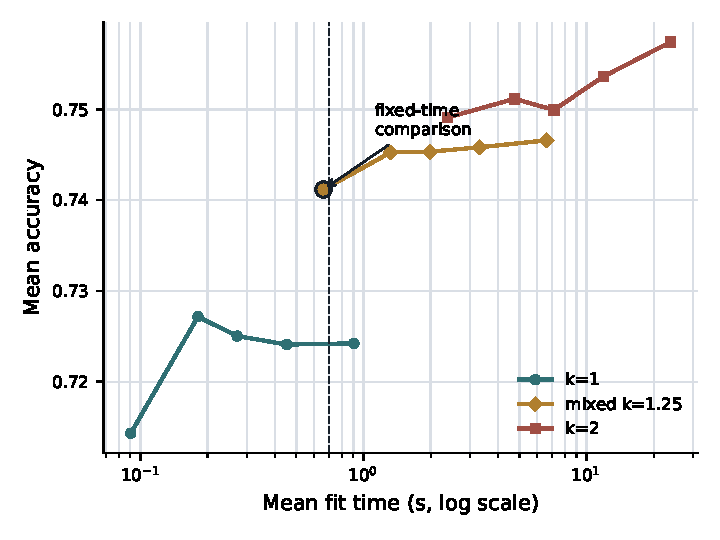
\includegraphics[width=4.8in]{Fig2_mixed_tradeoff.pdf}
\caption{Accuracy--time tradeoff for selected pure and mixed $k$-sighted forests on the 57-dataset mixed-forest benchmark. Each curve is evaluated at 20, 40, 60, 100, and 200 trees. The dashed vertical line marks a 0.7 s fitting-time budget.}
\label{fig:mixed}
\end{figure}

At the dashed budget line in Figure~\ref{fig:mixed}, the 20-tree $\bar{k}=1.25$ forest reaches 0.7412 mean accuracy in 0.661 s. Lower-sight forests at comparable times are less accurate: the 40-tree $\bar{k}=1.10$ forest reaches 0.7368 accuracy in 0.638 s, and the 60-tree $\bar{k}=1.05$ forest reaches 0.7340 accuracy in 0.614 s. This is not a tuned Pareto-frontier claim, but it is the clearest evidence in the benchmark that a few farther-sighted trees can help more than spending the same budget only on additional low-sight trees.

\section{Discussion}

The empirical message is conservative. Multi-step split optimization can improve shallow classification trees, but uniform non-greediness is costly and inconsistent. Greedy induction remains a strong accuracy--time compromise for single trees and for uniformly sighted forests. The useful exception is heterogeneous allocation: sparse $k=2$ trees can sometimes lift an otherwise greedy forest at a comparable fitting-time budget.

These experiments should not be read as a complete ranking of ensemble designs. They use one train--test split per dataset, shallow trees, all predictors at each split, and wall-clock times from one implementation. They also focus on classification benchmarks rather than targeted interaction problems. The result is nevertheless informative for tree design. If extra computation is available, the first practical question may not be whether every tree should be farther-sighted. It may be whether a small minority of farther-sighted trees diversifies a mostly greedy ensemble enough to justify its cost.

\section{Data availability}

The benchmark datasets are public PMLB datasets. Retained result tables supporting the article's tables and figures are supplied as supplementary review materials and can be regenerated from public data. To preserve double-blind review, the public repository link is omitted from this anonymized manuscript and will be inserted before publication.

\section{Code availability}

The custom code implementing $k$-sighted induction and generating the benchmark outputs is available to editors and reviewers upon request during peer review. It will be released in a public repository with reproduction documentation before publication.

\begin{thebibliography}{}

\bibitem[AGHAEI, G{\'O}MEZ, and VAYANOS(2025)]{aghaei2025strong}
AGHAEI, S., G{\'O}MEZ, A., and VAYANOS, P. (2025),
``Strong Optimal Classification Trees,''
\emph{Operations Research}, 73, 2223--2241.

\bibitem[BERTSIMAS and DUNN(2017)]{bertsimas2017optimal}
BERTSIMAS, D., and DUNN, J. (2017),
``Optimal Classification Trees,''
\emph{Machine Learning}, 106, 1039--1082.

\bibitem[BREIMAN(1996)]{breiman1996bagging}
BREIMAN, L. (1996),
``Bagging Predictors,''
\emph{Machine Learning}, 24, 123--140.

\bibitem[BREIMAN(2001)]{breiman2001random}
BREIMAN, L. (2001),
``Random Forests,''
\emph{Machine Learning}, 45, 5--32.

\bibitem[BREIMAN et al.(1984)]{breiman1984cart}
BREIMAN, L., FRIEDMAN, J. H., OLSHEN, R. A., and STONE, C. J. (1984),
\emph{Classification and Regression Trees},
Belmont, CA: Wadsworth.

\bibitem[ELOMAA and MALINEN(2005)]{elomaa2005lookahead}
ELOMAA, T., and MALINEN, T. (2005),
``On Look-Ahead and Pathology in Decision Tree Learning,''
\emph{Journal of Experimental \& Theoretical Artificial Intelligence}, 17, 19--33.

\bibitem[ESMEIR and MARKOVITCH(2007)]{esmeir2007anytime}
ESMEIR, S., and MARKOVITCH, S. (2007),
``Anytime Learning of Decision Trees,''
\emph{Journal of Machine Learning Research}, 8, 891--933.

\bibitem[HU, RUDIN, and SELTZER(2019)]{hu2019optimal}
HU, X., RUDIN, C., and SELTZER, M. (2019),
``Optimal Sparse Decision Trees,''
\emph{Advances in Neural Information Processing Systems}, 32, 7265--7273.

\bibitem[HYAFIL and RIVEST(1976)]{hyafil1976constructing}
HYAFIL, L., and RIVEST, R. L. (1976),
``Constructing Optimal Binary Decision Trees is NP-Complete,''
\emph{Information Processing Letters}, 5, 15--17.

\bibitem[LIN et al.(2020)]{lin2020generalized}
LIN, J., ZHONG, C., HU, D., RUDIN, C., and SELTZER, M. (2020),
``Generalized and Scalable Optimal Sparse Decision Trees,''
\emph{Proceedings of Machine Learning Research}, 119, 6150--6160.

\bibitem[MURTHY and SALZBERG(1995)]{murthy1995lookahead}
MURTHY, S. K., and SALZBERG, S. L. (1995),
``Lookahead and Pathology in Decision Tree Induction,''
\emph{Proceedings of the Fourteenth International Joint Conference on Artificial Intelligence}, 1025--1031.

\bibitem[NOROUZI et al.(2015)]{norouzi2015efficient}
NOROUZI, M., COLLINS, M. D., JOHNSON, M. A., FLEET, D. J., and KOHLI, P. (2015),
``Efficient Non-Greedy Optimization of Decision Trees,''
\emph{Advances in Neural Information Processing Systems}, 28, 1729--1737.

\bibitem[NORTON(1989)]{norton1989generating}
NORTON, S. W. (1989),
``Generating Better Decision Trees,''
\emph{Proceedings of the Eleventh International Joint Conference on Artificial Intelligence}, 800--805.

\bibitem[OLSON et al.(2017)]{olson2017pmlb}
OLSON, R. S., LA CAVA, W., ORZECHOWSKI, P., URBANOWICZ, R. J., and MOORE, J. H. (2017),
``PMLB: A Large Benchmark Suite for Machine Learning Evaluation and Comparison,''
\emph{BioData Mining}, 10, Article 36.

\bibitem[QUINLAN(1986)]{quinlan1986induction}
QUINLAN, J. R. (1986),
``Induction of Decision Trees,''
\emph{Machine Learning}, 1, 81--106.

\end{thebibliography}

\end{document}
